\documentclass[tikz,border=10pt]{standalone}
\usepackage[T1]{fontenc}
\usepackage{mathpazo}
\usepackage{amsmath,amssymb}
\usetikzlibrary{arrows.meta, positioning, calc, shapes.geometric}

\definecolor{stblue}{HTML}{7B97AD}
\definecolor{rwgold}{HTML}{B8995E}
\definecolor{sage}{HTML}{7A9A7E}
\definecolor{dkbrown}{HTML}{3D3530}
\definecolor{wmgray}{HTML}{7B7067}
\definecolor{cream}{HTML}{F9F6F0}
\definecolor{border}{HTML}{D4C9B8}

\begin{document}
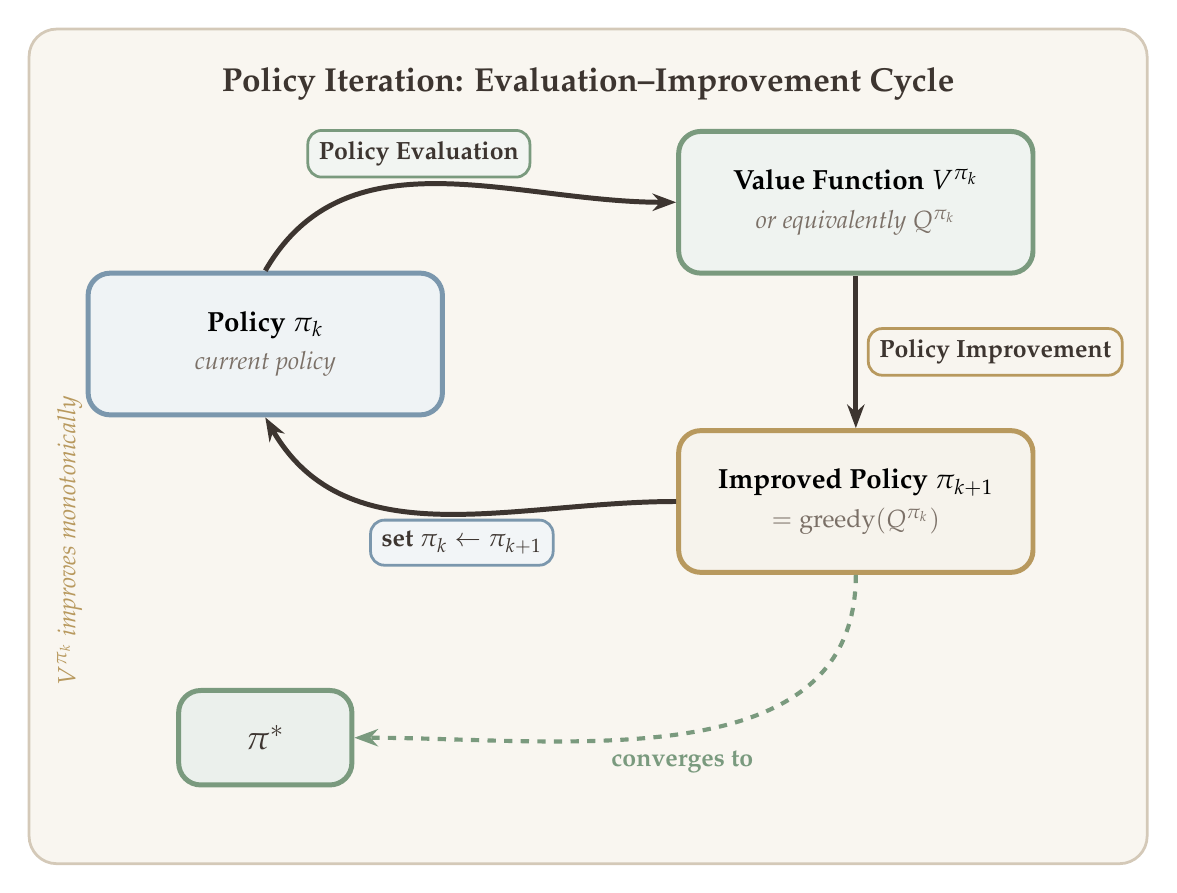
\begin{tikzpicture}[
  >={Stealth[length=3mm, width=2.2mm]},
  mainbox/.style={draw=#1, line width=1.8pt, fill=#1!12, rounded corners=8pt,
    minimum width=45mm, minimum height=18mm, align=center, inner sep=5pt},
  stepbox/.style={draw=#1, line width=1pt, fill=#1!10, rounded corners=5pt,
    font=\small\bfseries, text=dkbrown, inner sep=4pt},
  arr/.style={->, line width=1.8pt, dkbrown},
]

% Background
\fill[cream, rounded corners=10pt] (-5.0,-5.6) rectangle (9.2,5.0);
\draw[border, rounded corners=10pt, line width=1pt] (-5.0,-5.6) rectangle (9.2,5.0);

% Title
\node[font=\large\bfseries, text=dkbrown] at (2.1,4.3)
  {Policy Iteration: Evaluation--Improvement Cycle};

% === Three main boxes ===

% Policy pi_k (left)
\node[mainbox=stblue] (policy) at (-2.0,1.0)
  {\textbf{Policy $\pi_k$}\\[2pt]
   {\small\itshape\color{wmgray} current policy}};

% Value function (top right)
\node[mainbox=sage] (value) at (5.5,2.8)
  {\textbf{Value Function $V^{\pi_k}$}\\[2pt]
   {\small\itshape\color{wmgray} or equivalently $Q^{\pi_k}$}};

% Improved policy (bottom right)
\node[mainbox=rwgold] (improved) at (5.5,-1.0)
  {\textbf{Improved Policy $\pi_{k+1}$}\\[2pt]
   {\small\itshape\color{wmgray} $= \operatorname{greedy}(Q^{\pi_k})$}};

% === Arrows with labels ===

% Arrow 1: Policy -> Value (Policy Evaluation)
\draw[arr] (policy.north) to[out=60, in=180]
  node[stepbox=sage, pos=0.45, above=2pt] {Policy Evaluation}
  (value.west);

% Arrow 2: Value -> Improved (Policy Improvement)
\draw[arr] (value.south) --
  node[stepbox=rwgold, right=4pt] {Policy Improvement}
  (improved.north);

% Arrow 3: Improved -> Policy (loop back)
\draw[arr] (improved.west) to[out=180, in=-60]
  node[stepbox=stblue, pos=0.45, below=2pt]
    {set $\pi_k \gets \pi_{k+1}$}
  (policy.south);

% === Convergence to pi* ===
\node[draw=sage, line width=1.8pt, fill=sage!15, rounded corners=8pt,
  minimum width=22mm, minimum height=12mm,
  font=\large\bfseries, text=dkbrown] (pistar) at (-2.0,-4.0) {$\pi^*$};

\draw[->, line width=1.5pt, sage, dashed]
  (improved.south) to[out=-90, in=0]
  node[pos=0.5, below=2pt, font=\small\bfseries, text=sage] {converges to}
  (pistar.east);

% === Monotone improvement annotation ===
\node[font=\small\itshape, text=rwgold, rotate=90, anchor=south] at (-4.2,-1.5)
  {$V^{\pi_k}$ improves monotonically};

\end{tikzpicture}
\end{document}
